% ----------------------------------------------------------
\chapter{METODOLOGIA}
% ----------------------------------------------------------


Este trabalho foi baseado na pesquisa de Zhang et al. (2020a), cujos autores resolvem um modelo numérico de compressor linear completo (sistemas elétrico, mecânico,  termodinâmico) utilizando o software PDSim (BELL et al., 2020). Neste trabalho optou-se por desenvolver o submodelo em uma linguagem de programação amplamente utilizada a fim de futuramente acoplá-los a um software de simulação termodinâmico existente implementado em C++.

Nesta seção serão apresentadas as etapas de implementação do algoritmo para a integração dos submodelos desenvolvidos e os submodelos desenvolvidos: mecânico, elétrico e termodinâmico. Para que a implementação numérica fosse possível, este estudo se deu com uso do software Matlab e da biblioteca termodinâmica CoolProp, desenvolvida por Bell et al. (2014).

Os resultados obtidos por Zhang et al. (2020a) serão utilizados como comparação para o modelo desenvolvido. Entretanto, deve-se salientar que o submodelo termodinâmico de Zhang et al. (2020a) inclui efeitos de vazamento, transferência de calor e movimento de válvulas, por exemplo. Tais efeitos tornam a simulação mais verossímil quando comparada com um ciclo de compressão ideal. Levando isso em conta, espera-se que haja alguma divergência nos resultados quando as comparações envolverem os submodelos termodinâmicos.

\section{GEOMETRIA E DADOS DO COMPRESSOR}

Com a geometria definida é possível encontrar dados importantes, como volume da câmara de compressão, área do pistão, valor da massa efetiva e dados sobre o circuito elétrico do motor. Tais dados serão usados para a resolução dos submodelos mecânico e elétrico, e estão dispostos na Tabela \ref{tab:Tab_1} :







\begin{table}[htb]
	\ABNTEXfontereduzida
	\caption{\label{tab:Tab_1} Dados da geometria e motor para o compressor}
	\begin{center}
	\begin{tabular}{p{5.0cm}p{1.5cm}p{2cm}p{2.5cm}}
		\toprule
		\textbf{Parâmetro} &  \textbf{Símbolo}      & \textbf{Valor} & \textbf{Unidade}    \\ \midrule
	Diâmetro do pistão                 & $D_p$              & 26,5              & $mm$                                      \\
		Massa do pistão                    & $m_p$          & 0,632            & $kg$                                        \\
		Massa das molas                    & $m_s$          & 0,164             & $kg$                                       \\
		Constante de rigidez das molas     & $k_s$          & 45,66             & $Nmm^{-1}$                                  \\
        Fator de motor                     & $\alpha$       & 75             & $NA^{-1}$                                        \\ 
		Resistência elétrica do motor      & $\Omega$       & 15,7             & $\Omega$                                     \\ 
		Indutância do motor                & $L$            & 450             & $mH$                                            \\ \bottomrule
	\end{tabular}
	\end{center}
	\fonte{Adaptado de Zhang et al. (2020)}
\end{table}

O dado da capacitância não foi apresentado em Zhang et al. (2020a). Esse dado foi calculado utilizando a Equação 9, com os valores de R, L e as curvas de deslocamento e corrente fornecidas nos resultados de Zhang et al. (2020a). Para um dado instante de tempo é possível encontrar os valores para todos os elementos da Equação 9 menos a capacitância, assim isolando-a e encontrando seu valor. Neste caso o valor encontrado foi de C = 35F.

\section{CONDIÇÕES DE OPERAÇÃO}

A condição de operação pode ser descrita pelos parâmetros listados na Tabela \ref{tab:Tab_2}. Tais dados foram retirados da Tabela 3.1 de Zhang et al. (2020), com exceção do valor da razão de pressões, PR. 



\begin{table}[htb]
	\ABNTEXfontereduzida
	\caption{\label{tab:Tab_2}Condições de operação para o compressor}
	\begin{center}
	\begin{tabular}{p{5.0cm}p{1.5cm}p{2cm}p{2.5cm}}
		\toprule
		\textbf{Parâmetro} &  \textbf{Símbolo}      & \textbf{Valor} & \textbf{Unidade}    \\ \midrule
	    Fluido de trabalho              & -              & R134a        & -                                      \\
		Pressão de sucção               & $P_{suc}$          & 111,81   & $Pa$                                        \\
		Temperatura de Sucção           & $T_{suc}$          & 8,08     & $°C$                                       \\
        Razão de pressões               & $PR$       & 4,9              & -                                        \\ 
		Frequência de operação          & $f$       & 60                & $Hz$                                     \\  \bottomrule
	\end{tabular}
	\end{center}
	\fonte{Adaptado de Zhang et al. (2020)}
\end{table}


O valor da razão de pressões de Zhang et al. (2020a) descrito em seu artigo é 5,5. Porém, analisando os resultados de Zhang et al (2020a), que apresenta valores para pressão na câmara de compressão, e com ajuda da plataforma online WebPlotDigitalizer (ROHATGI, 2020), é possível perceber que pressão descarga é igual a, aproximadamente, 4,9 vezes maior que a pressão de sucção.

%\begin{figure}[htb]
%	\caption{\label{fig:zhang_pressao}Gráfico do resultado de Zhang et al. (2020a) em regime permanente da pressão no cilindro em função do tempo.}
%	\begin{center}
%		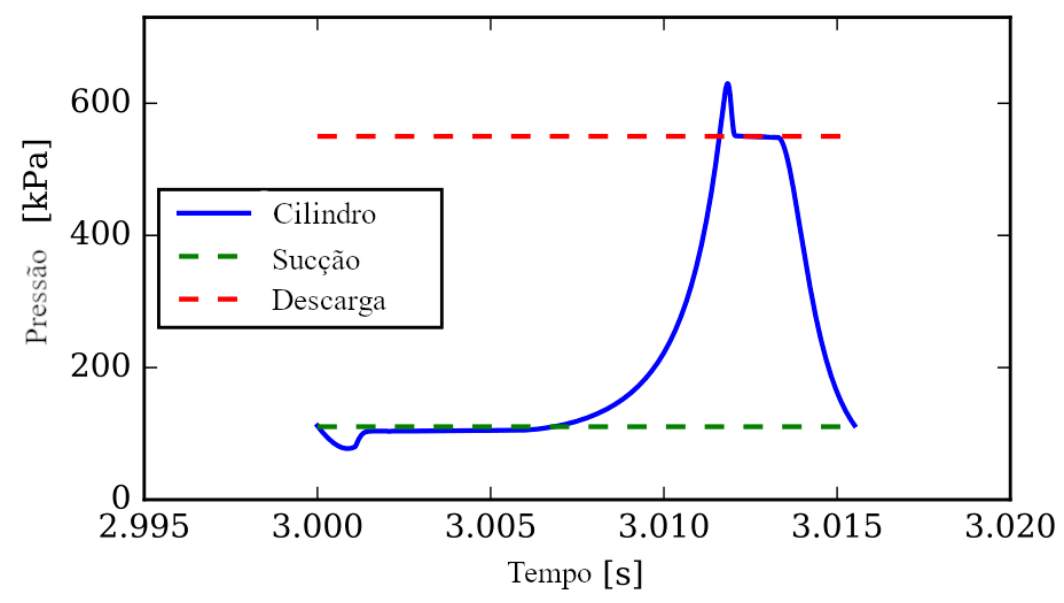
\includegraphics[scale=0.4]{images/pressao_zhang.png}
%	\end{center}
%	\fonte{Adaptado de Zhang et al. (2020)}
%\end{figure}

%Ainda analisando a Figura \ref{fig:zhang_pressao}, o dado apresentado pelo autor para PR = 5,5 não condiz com o apresentado em seu resultado. Por esse motivo se fez necessário e justificável realizar esta alteração nos dados da referência.

\section{MODELO NUMÉRICO}

A modelagem numérica de um problema representa, de forma simplificada, o processo de algum fenômeno. No caso de um compressor linear, é preciso levar em conta três submodelos: (i) o elétrico, que determina a força eletromagnética agindo sobre o magneto a partir de dados de tensão de entrada e movimento do pistão; (ii) o mecânico, que determina a posição do pistão a partir de todas as excitações sofridas; e (iii) o termodinâmico, que calcula o esforço exercido pelo gás comprimido sobre o pistão.


\subsection{Submodelo elétrico}

É prática comum na literatura representar o motor de um compressor linear como um circuito RLC (Zhang et al., 2020a; Bijanzad et al., 2020a), consistindo de um resistor, um indutor e um capacitor ligados em série com uma fonte de tensão (Figura \ref{fig:circuito-eletrico}). Resultados obtidos por Zhang et al. (2020b) foram inclusive utilizados para validar este modelo.

\begin{figure}[htb]
	\caption{\label{fig:circuito-eletrico} Diagrama do circuito elétrico usado em compressores lineares.}
	\begin{center}
		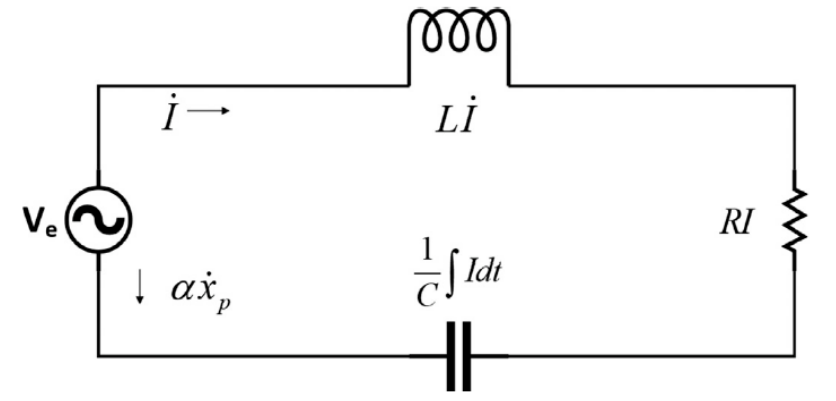
\includegraphics[scale=0.65]{images/circuito.png}
	\end{center}
	\fonte{Adaptado de Zhang et al. (2021)}
\end{figure}

Na Figura \ref{fig:circuito-eletrico}, a variável I, representa a corrente elétrica , R a resistência ,L a indutância, C a capacitância ,t o tempo ,Ve a tensão alternada e uemft é a força eletromotriz inversa, que é proveniente da própria Lei de Faraday aplicada. Essa força ocorre normalmente em motores elétricos devido ao movimento relativo do magneto, que gera uma diferença de potencial. O equacionamento do circuito pode ser obtido a partir das leis de Kirchhoff como mostrado na Equação \ref{eq:eletrico}: 




\begin{equation}\label{eq:eletrico}
V_e-u_{emf}(t)= LI'+RI+\frac{1}{C} \int I \,dt ,
\end{equation}


onde $u_{emf}(t)$ é definido a partir da Lei de Faraday:




\begin{equation}\label{eq:uemf}
u_{emf}(t)=Blx'_p= x'p.
\end{equation}


Nesta Equação \ref{eq:uemf}, B é a densidade magnética das bobinas, l o tamanho do condutor, e , que é o produto de B e l, é o fator de motor. Além desses parâmetros, a velocidade instantânea do pistão entra no cálculo como x'p.
A potência elétrica consumida pelo motor pode ser calculada a partir da Equação 11:

\begin{equation}\label{eq:uemf}
W_{e} = f \int_{0}^{1/f} V_eI(t)\,dt
\end{equation}


\subsection{Submodelo mecânico}

No caso do modelo mecânico, o mecanismo é tratado como um sistema massa-mola-amortecedor. Nesse caso, o diagrama de corpo livre do pistão pode ser observado na Figura \ref{fig:forcas-atuando}. A variável $P(t)$ representa a pressão na câmara de compressão, $P_{shell}$ é a pressão de sucção existente no ambiente interno do compressor, $A_p$ é a área da seção transversal do pistão, $k_s$ é a constante de rigidez da mola, $c_{fri}$ é o coeficiente de fricção, $I(t)$ representa a corrente elétrica instantânea,  é o fator de motor, e $x_p$,$x^{'} _p$ e $x{''} _p$ representam o deslocamento, velocidade e aceleração do pistão, respectivamente. Reunindo todos esses termos e aplicando a segunda Lei de Newton obtém-se:


\begin{figure}[htb]
	\caption{\label{fig:forcas-atuando} Representação das forças atuando no pistão.}
	\begin{center}
		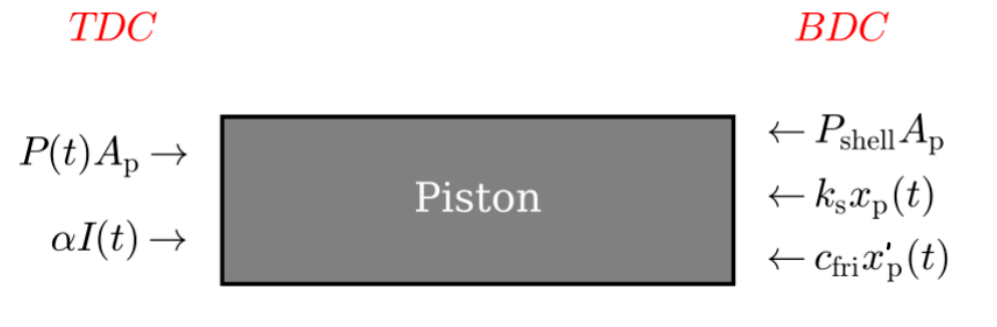
\includegraphics[scale=0.65]{images/pistao.png}
	\end{center}
	\fonte{Adaptado de Zhang et al. (2020a)}
\end{figure}

\begin{equation}\label{eq:mecanico}
m_{eff}x''_p + c_{fri}x'_p+ k_{s}x_p + (P_shell - P(t))A_p = \alpha I(t) 
\end{equation}

A Equação \ref{eq:mecanico} representa a equação de movimento do pistão, onde $m_{eff}$ é a massa efetiva do sistema.

%Na Figura \ref{fig:dados_ref} é possível ver o pistão dentro do cilindro. TDC significa \textit{Top Dead Center}, do inglês, BDC é o \textit{Bottom Dead Center}. $X_m$é a posição sobre a qual o sistema oscila harmonicamente, esse valor pode variar conforme o carregamento dinâmico no pistão é alterado. $X_0$ é a distância fixa entre a placa da válvula de descarga e o topo do pistão quando não há nenhum carregamento dinâmico atuando no pistão. 


%\begin{figure}[htb]
%	\caption{\label{fig:dados_ref}Descrição de dados para referência no cálculo do pistão.}
%	\begin{center}
%		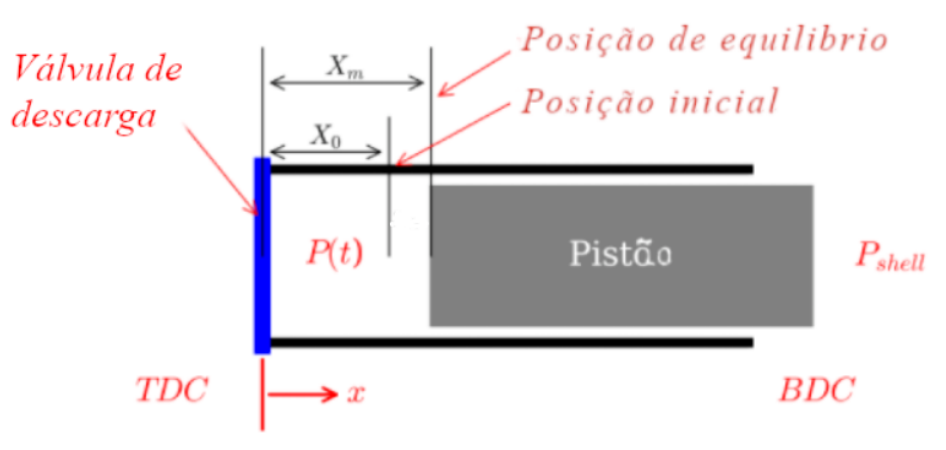
\includegraphics[scale=0.65]{images/pistao_02.png}
%	\end{center}
%	\fonte{Adaptado de Zhang et al. (2021)}
%\end{figure}

%O volume na câmara de compressão é calculado pela  Equação \ref{eq:volume}:


%\begin{equation}\label{eq:volume}
% V= x_{rp}A_p,
%\end{equation}

%onde $x_{rp}$ é definido na Equação \ref{eq:xrp}: 

%\begin{equation}\label{eq:xrp}
%x_{rp} = x_p + X_0,
%\end{equation}
%e $x_p$ é a posição de deslocamento do pistão em relação a $X0$.
%Em algumas situações específicas, observou-se que o carregamento de pressão sobre o pistão poderia ocasionar valores negativos de xrp,fazendo com que o volume da câmara de compressão fosse negativo e gerando erros na simulação. Essa condição foi observada durante o transiente inicial do compressor e em determinadas condições de operação nas quais a posição de equilíbrio fica muito próxima da placa de válvulas. A fim de evitar erros na simulação, decidiu-se implementar uma força de mola fictícia ao pistão  quando ele passa de um determinado volume mínimo. Essa força pode ser vista na Equação 15:

%\begin{equation}\label{eq:f_virt}
%F_{a} = k_{virtual}max( 0 , 0.0004 - X_0 - x_p),
%\end{equation}
%onde kvirtual foi adotado igual a 5,106 N/m. A força $Fa$, atua no sentido positivo do eixo x, tendendo a afastar o pistão da placa de válvulas.  Ainda com relação a Equação \ref{eq:f_virt}, é necessário deixar bem claro que essa adaptação só passa a ocorrer caso o pistão esteja a uma distância inferior a 0,0004 m da placa de válvulas.

A potência mecânica, transmitida pelo motor ao pistão pode ser calculada como:


\begin{equation}\label{eq:f_virt}
W_{m} = f \int_{0}^{1/f} I(t)x'_p(t) \,dt
\end{equation}

\subsection{Submodelo termodinâmico}

Este trabalho tem como foco a implementação dos submodelos elétrico e mecânico, embora seja necessário um submodelo termodinâmico para prever o carregamento de pressão sobre o pistão. Logo, optou-se pelo submodelo termodinâmico mais simples possível, ou seja, o ciclo ideal de compressão de vapor foi considerado, sendo compreendido por processos de expansão e compressão isentrópicos e processos de sucção e descarga isobáricos (Figura \ref{fig:grafico_pv}).


\begin{figure}[htb]
	\caption{\label{fig:grafico_pv}Diagrama Pressão-Volume do ciclo ideal de compressão de vapor com a explicação de cada ciclo e o sentido.}
	\begin{center}
		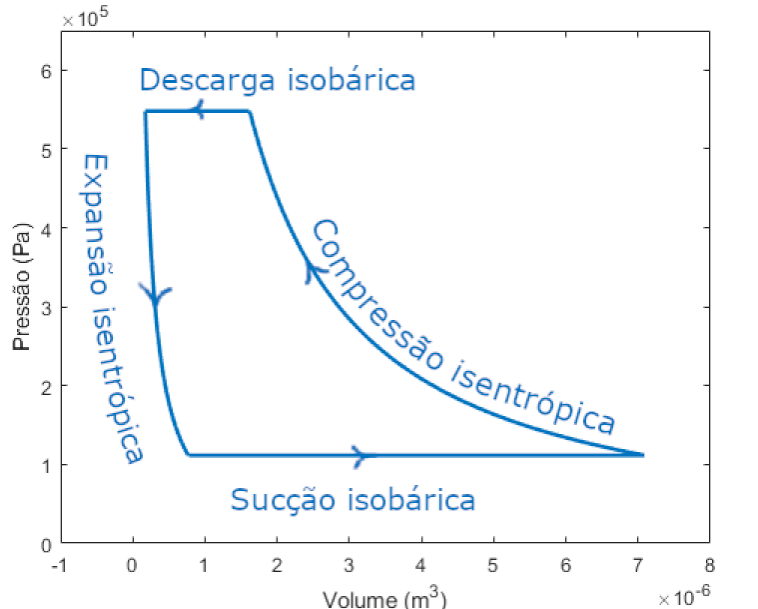
\includegraphics[scale=0.50]{images/termodinamico.png}
	\end{center}
	\fonte{Autor (2021)}
\end{figure}

A potência termodinâmica, $W_t$, pode ser calculada a partir da integração do diagrama pressão-volume. Assim, as eficiências elétrica e mecânica podem ser obtidas a partir do acoplamento de todos os submodelos. A eficiência elétrica, $\eta_e$, representa a razão entre a potência mecânica, $W_m$, e a potência elétrica, $W_e$, enquanto a eficiência mecânica, $\eta_m$, representa a razão entre a potência termodinâmica e a potência mecânica.

\section{RESOLUÇÃO DAS EQUAÇÕES}

O problema apresenta três submodelos, e dois deles envolvem equações diferenciais ordinárias de segunda ordem, representada pelas Equações 9 e 12, sendo, respectivamente, os submodelos elétrico e mecânico. Essas equações foram resolvidas utilizando o método de Runge Kutta de 4ª ordem.
Na Figura \ref{fig:fluxograma}, é possível observar todas as etapas da metodologia de resolução adotada. 

\begin{figure}[htb]
	\caption{\label{fig:fluxograma}Fluxograma da linha de cálculo do algoritmo.}
	\begin{center}
		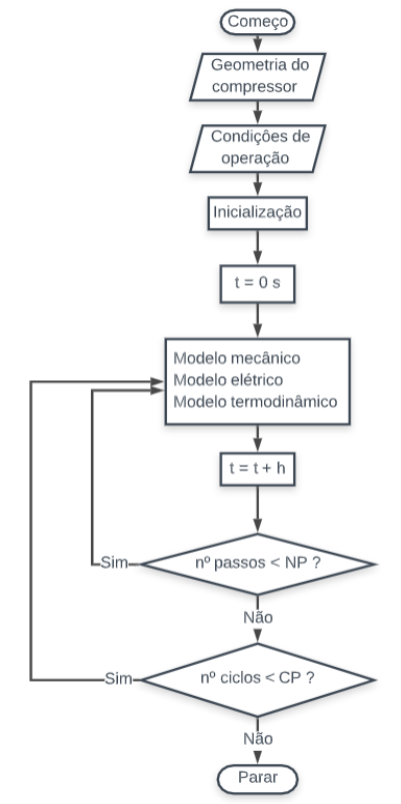
\includegraphics[scale=0.65]{images/modelo_geral.png}
	\end{center}
	\fonte{Autor (2021)}
\end{figure}


A Figura \ref{fig:fluxograma} mostra a lógica adotada, onde “CP” é o número total de passos que cada ciclo tem e “NP”  é o número total de passos, caso o valor não tenha atingido o número total de de passos do ciclo ele retorna ao looping, caso esses valores sejam iguais, o código avança para o próximo ciclo, assim até completar o número de ciclos desejados. No caso deste trabalho o número de passos, CP, é 1000 e o número de ciclos, NP, 100.
A única variável de entrada é o valor da tensão, que foi definida a partir dos resultados de Zhang et al. (2020), sendo mostrada na Equação \ref{eq:ve} : 


\begin{equation}\label{eq:ve}
V_e(t)=220cos(2\pi60t)
\end{equation}

\vfill \break


É possível observar na Equação \ref{eq:ve} que a frequência de oscilação é igual a 60 Hz e uma tensão alternada de 220 V, em outras palavras, é uma tensão nominal comum numa residência.

%A Figura \ref{fig:rk} é um esquemático do acontece dentro do método de Runge-Kutta aplicado, cada submodelo é dependente do outro. A cada loop feito representa um passo de tempo h fixo, a duração do ciclo é definida pela frequência dada T =1/f   e o passo é definido h=T/NC onde NC é um número pré-definido pelo usuário. A quantidade de ciclos feitos também é um dado que o usuário pode escolher.


%\begin{figure}[htb]
%	\caption{\label{fig:rk}Esquema de resolução dentro do método de Runge-Kutta}
%	\begin{center}
%		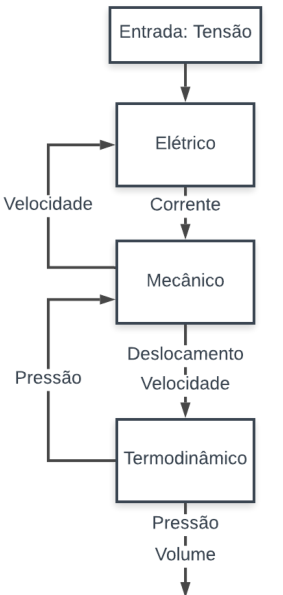
\includegraphics[scale=0.70]{images/modelo_rk.png}
%	\end{center}
%	\fonte{Autor (2021)}
%\end{figure}

%Percebe-se pela Figura \ref{fig:rk} que cada submodelo é dependente do outro: o elétrico depende da velocidade do pistão, pois ocorre o efeito da Lei de Faraday. O mecânico depende da pressão na câmara de compressão do termodinâmico e da corrente do elétrico. O termodinâmico depende da velocidade e deslocamento do pistão do mecânico. E dessa forma os submodelos se integram e formam o modelo desenvolvido.
